
%(BEGIN_QUESTION)
% Copyright 2015, Tony R. Kuphaldt, released under the Creative Commons Attribution License (v 1.0)
% This means you may do almost anything with this work of mine, so long as you give me proper credit

The following diagrams document the overcurrent protection system for a feeder supplying three-phase AC power to an industrial load:

$$\includegraphics[width=15.5cm]{i01279x01.eps}$$

Suppose one day the circuit breaker (52) trips for no apparent reason.  None of the brightly-colored ``target'' flags on the electromechanical protective relay are visible, as one would normally expect following a relay trip event.  Identify the likelihood of each specified fault for this system.  Consider each fault one at a time (i.e. no coincidental faults), determining whether or not each fault could independently account for {\it all} measurements and symptoms in this circuit.

% No blank lines allowed between lines of an \halign structure!
% I use comments (%) instead, so that TeX doesn't choke.

$$\vbox{\offinterlineskip
\halign{\strut
\vrule \quad\hfil # \ \hfil & 
\vrule \quad\hfil # \ \hfil & 
\vrule \quad\hfil # \ \hfil \vrule \cr
\noalign{\hrule}
%
% First row
{\bf Fault} & {\bf Possible} & {\bf Impossible} \cr
%
\noalign{\hrule}
%
% Another row
Dead DC station power supply &  &  \cr
%
\noalign{\hrule}
%
% Another row
52/TC coil failed shorted &  &  \cr
%
\noalign{\hrule}
%
% Another row
51-3/SI coil failed shorted &  &  \cr
%
\noalign{\hrule}
%
% Another row
50-1 contact failed open &  &  \cr
%
\noalign{\hrule}
%
% Another row
50-1 contact failed shorted &  &  \cr
%
\noalign{\hrule}
%
% Another row
50-2 coil failed shorted &  &  \cr
%
\noalign{\hrule}
%
% Another row
50-2 coil failed open &  &  \cr
%
\noalign{\hrule}
} % End of \halign 
}$$ % End of \vbox

Also, identify which side of the 52 circuit breaker should be the ``line'' (supply) and which side should be the ``load'' in order for the 50/51 relay to provide maximum protection in this system.

\vfil 

\underbar{file i01279}
\eject
%(END_QUESTION)





%(BEGIN_ANSWER)

This is a graded question -- no answers or hints given!
 
%(END_ANSWER)





%(BEGIN_NOTES)

% No blank lines allowed between lines of an \halign structure!
% I use comments (%) instead, so that TeX doesn't choke.

$$\vbox{\offinterlineskip
\halign{\strut
\vrule \quad\hfil # \ \hfil & 
\vrule \quad\hfil # \ \hfil & 
\vrule \quad\hfil # \ \hfil \vrule \cr
\noalign{\hrule}
%
% First row
{\bf Fault} & {\bf Possible} & {\bf Impossible} \cr
%
\noalign{\hrule}
%
% Another row
Dead DC station power supply &  & $\surd$ \cr
%
\noalign{\hrule}
%
% Another row
52/TC coil failed shorted &  & $\surd$ \cr
%
\noalign{\hrule}
%
% Another row
51-3/SI coil failed shorted &  & $\surd$ \cr
%
\noalign{\hrule}
%
% Another row
50-1 contact failed open &  & $\surd$ \cr
%
\noalign{\hrule}
%
% Another row
50-1 contact failed shorted & $\surd$ &  \cr
%
\noalign{\hrule}
%
% Another row
50-2 coil failed shorted &  & $\surd$ \cr
%
\noalign{\hrule}
%
% Another row
50-2 coil failed open &  & $\surd$ \cr
%
\noalign{\hrule}
} % End of \halign 
}$$ % End of \vbox

For maximum protection the relay's zone of protection should include the circuit breaker.  This means the bottom side will be the line and the top side will be the load.  That way, if the circuit breaker suffers an internal fault, the relay (with its CTs being on the breaker's line side) will detect the overcurrent from that fault and trip the breaker.

%INDEX% Electric power systems: protective relays (time-overcurrent)
%INDEX% Protective relay: instantaneous overcurrent (50)
%INDEX% Protective relay: time-overcurrent (51)

%(END_NOTES)


